\section{Atividades}

Neste módulo, foram realizadas atividades práticas voltadas à administração
de armazenamento e proteção de dados em sistemas Linux utilizando o Kali
Linux. As tarefas envolveram a utilização da ferramenta \textit{Duplicity}
para criação de backups completos e diferenciais, além da exploração de
técnicas de formatação e sobrescrita segura de dados em partições de disco.

Também foram utilizados comandos de baixo nível do sistema, como
\textit{fdisk}, \textit{wipefs}, \textit{dd} e \textit{shred}, permitindo
compreender como funcionam processos de remoção segura de dados e
gerenciamento de partições no Linux. O objetivo foi demonstrar, na prática,
mecanismos utilizados tanto para proteção quanto para eliminação segura de
informações armazenadas.

\newpage

\question[Atividade 7.6]{Backup Completo Local com Duplicity no Kali Linux}

\begin{figure}[H]
  \centering
  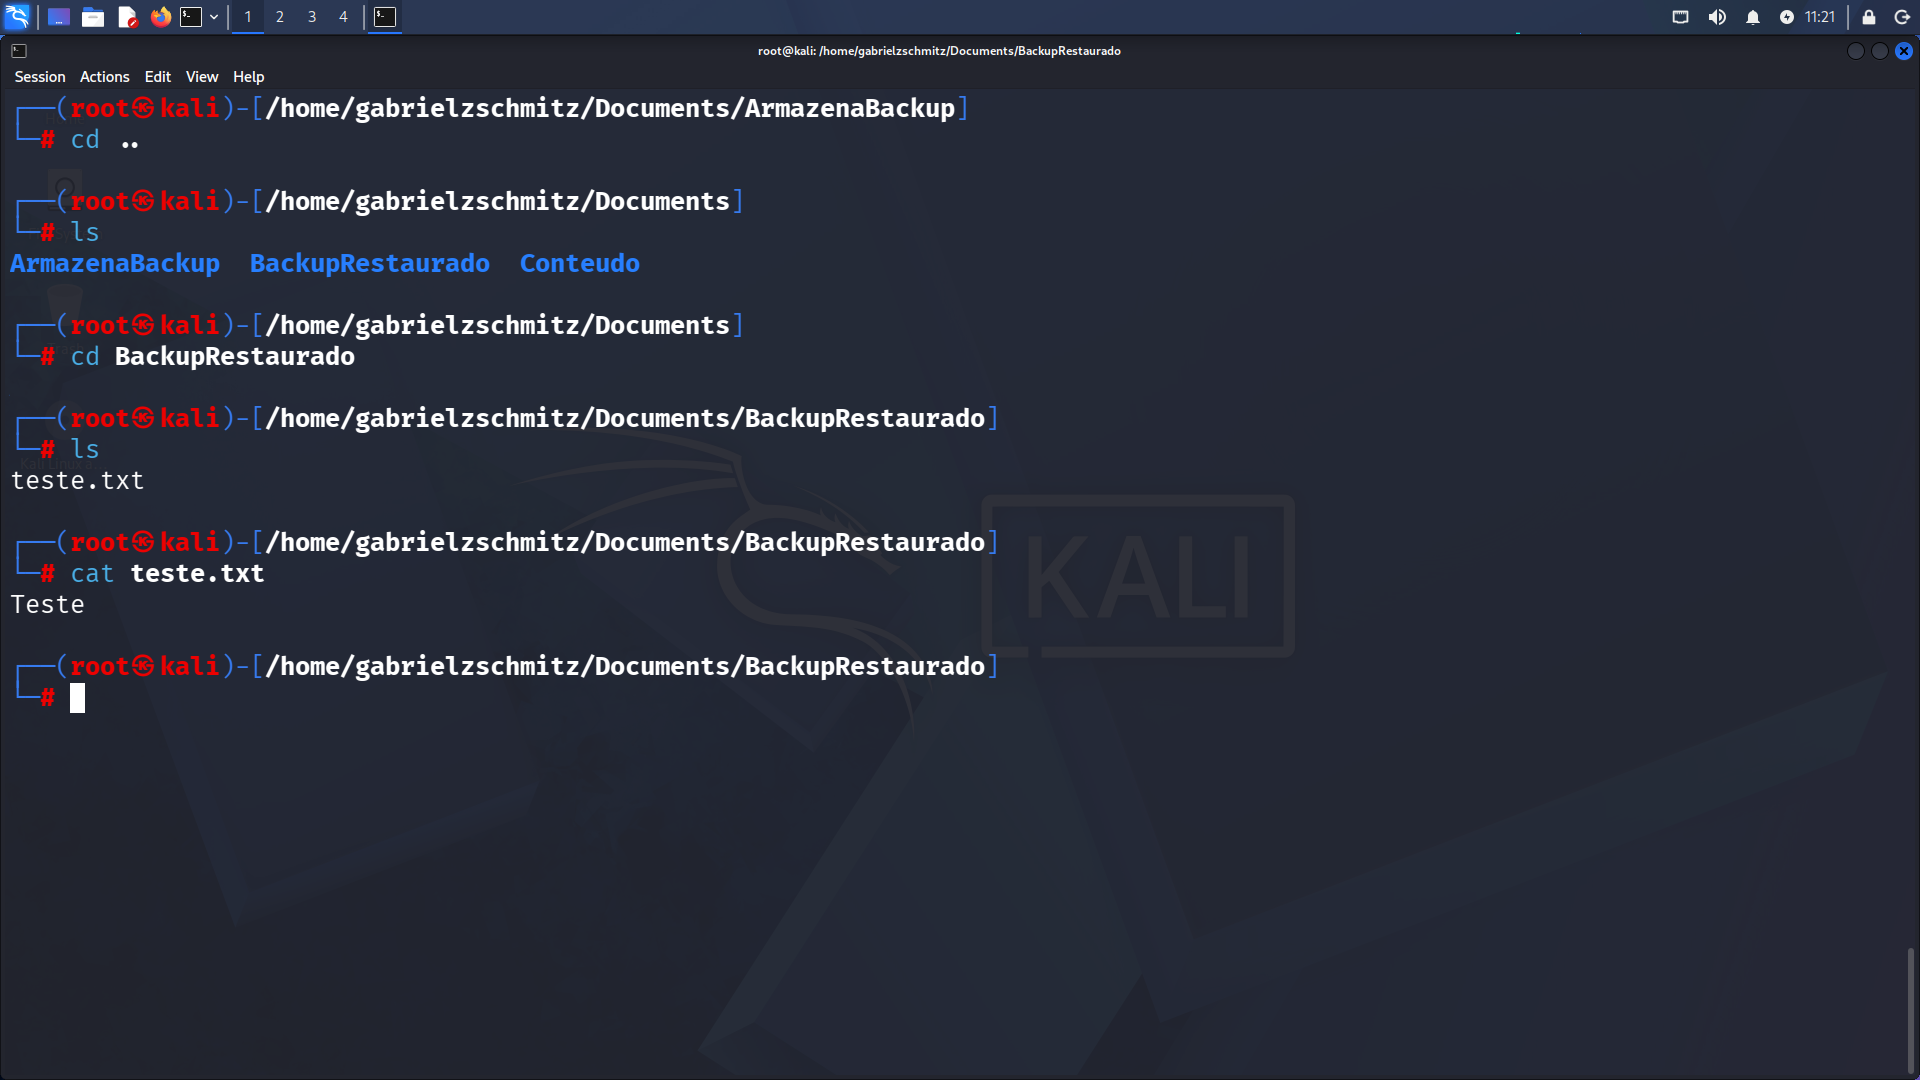
\includegraphics[width=0.99\textwidth]{./fig/fig7.6.png}
  \caption{Verificação do conteúdo restaurado após a execução do backup completo com Duplicity}
  \label{fig:fig7.6}
\end{figure}

\newpage

\question[Atividade 7.7]{Backup Diferencial Local com Duplicity no Kali Linux}

\begin{figure}[H]
  \centering
  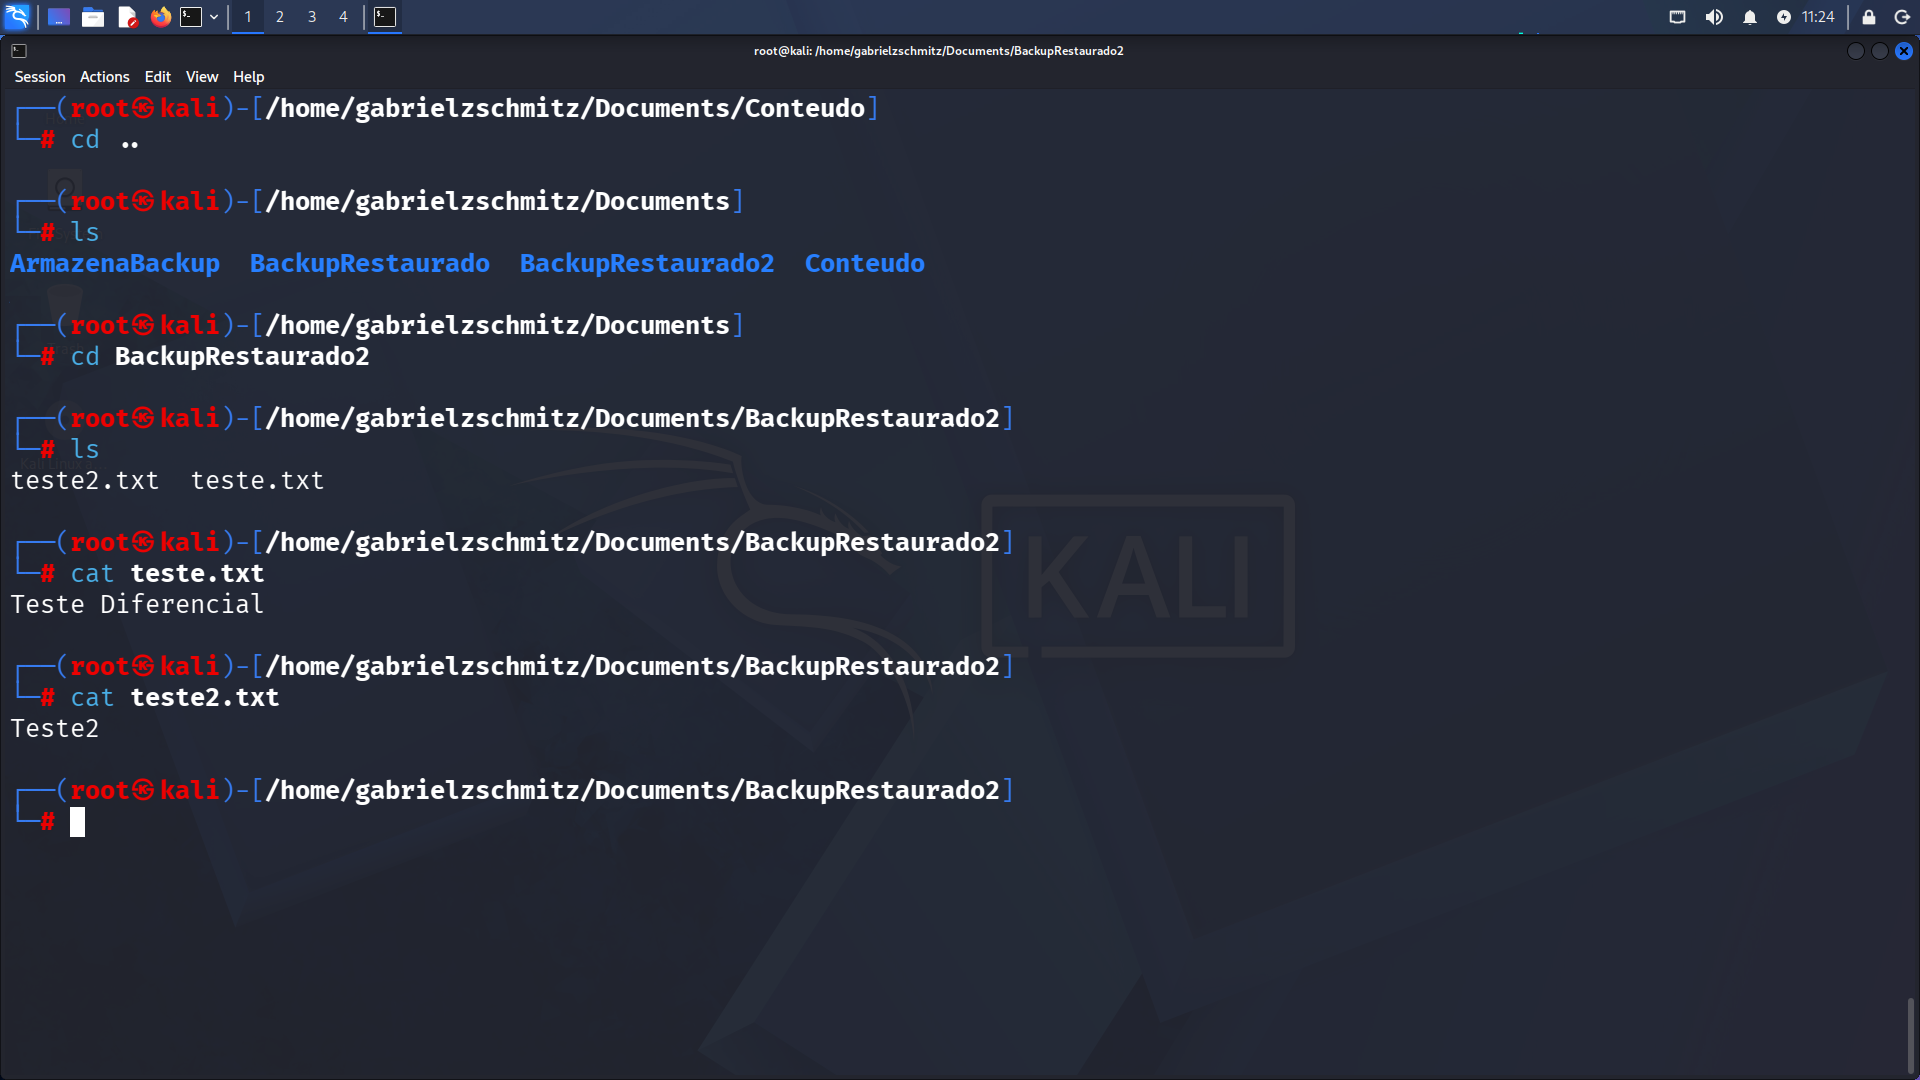
\includegraphics[width=0.99\textwidth]{./fig/fig7.7.png}
  \caption{Verificação da restauração do backup diferencial contendo os arquivos modificados}
  \label{fig:fig7.7}
\end{figure}

\newpage

\question[Atividade 7.8]{Formatação Completa de Partição no Kali Linux}

\begin{figure}[H]
  \centering
  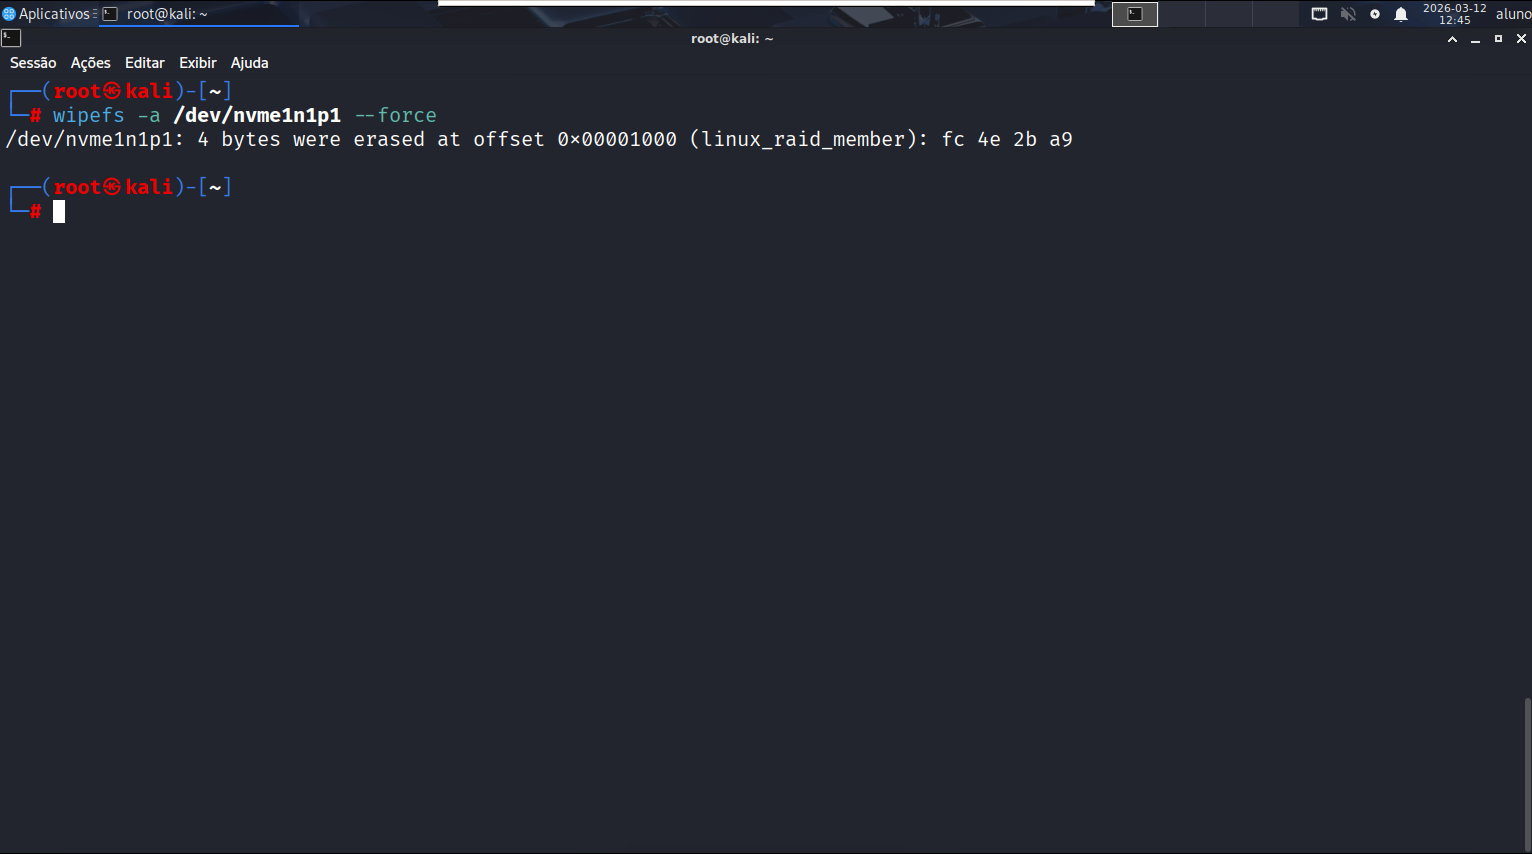
\includegraphics[width=0.99\textwidth]{./fig/fig7.8.png}
  \caption{Execução do comando wipefs removendo assinaturas de sistema de arquivos da partição}
  \label{fig:fig7.8}
\end{figure}

\newpage

\question[Atividade 7.9]{Sobrescrita Simples com Bits Aleatórios}

\begin{figure}[H]
  \centering
  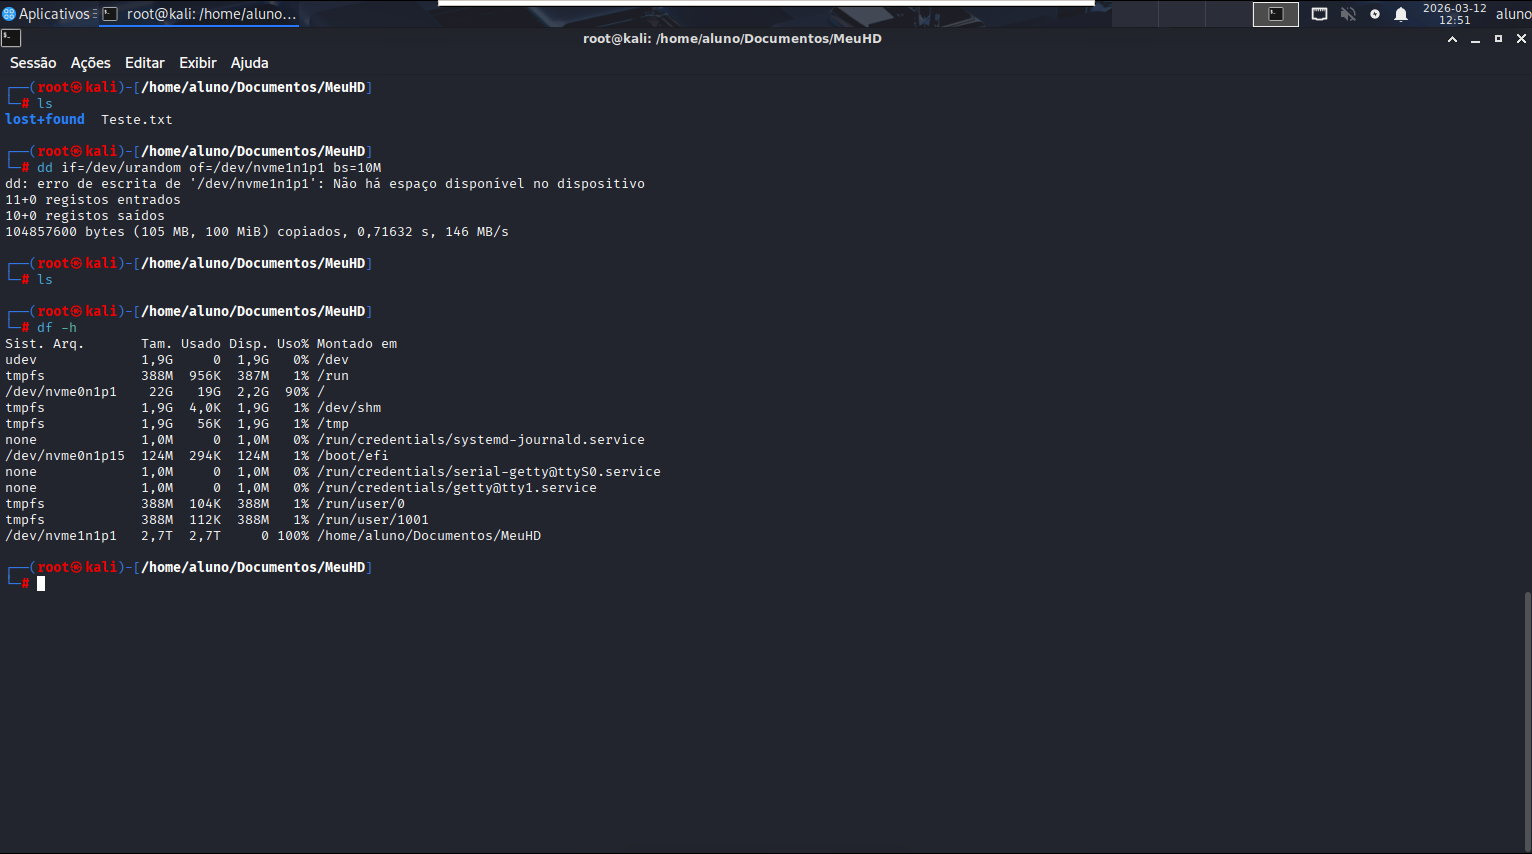
\includegraphics[width=0.99\textwidth]{./fig/fig7.9.png}
  \caption{Resultado do comando df -h demonstrando a partição totalmente preenchida após sobrescrita}
  \label{fig:fig7.9}
\end{figure}

\newpage

\question[Atividade 7.10]{Sobrescrita com o padrão DoD 5220.22-M}

\begin{figure}[H]
  \centering
  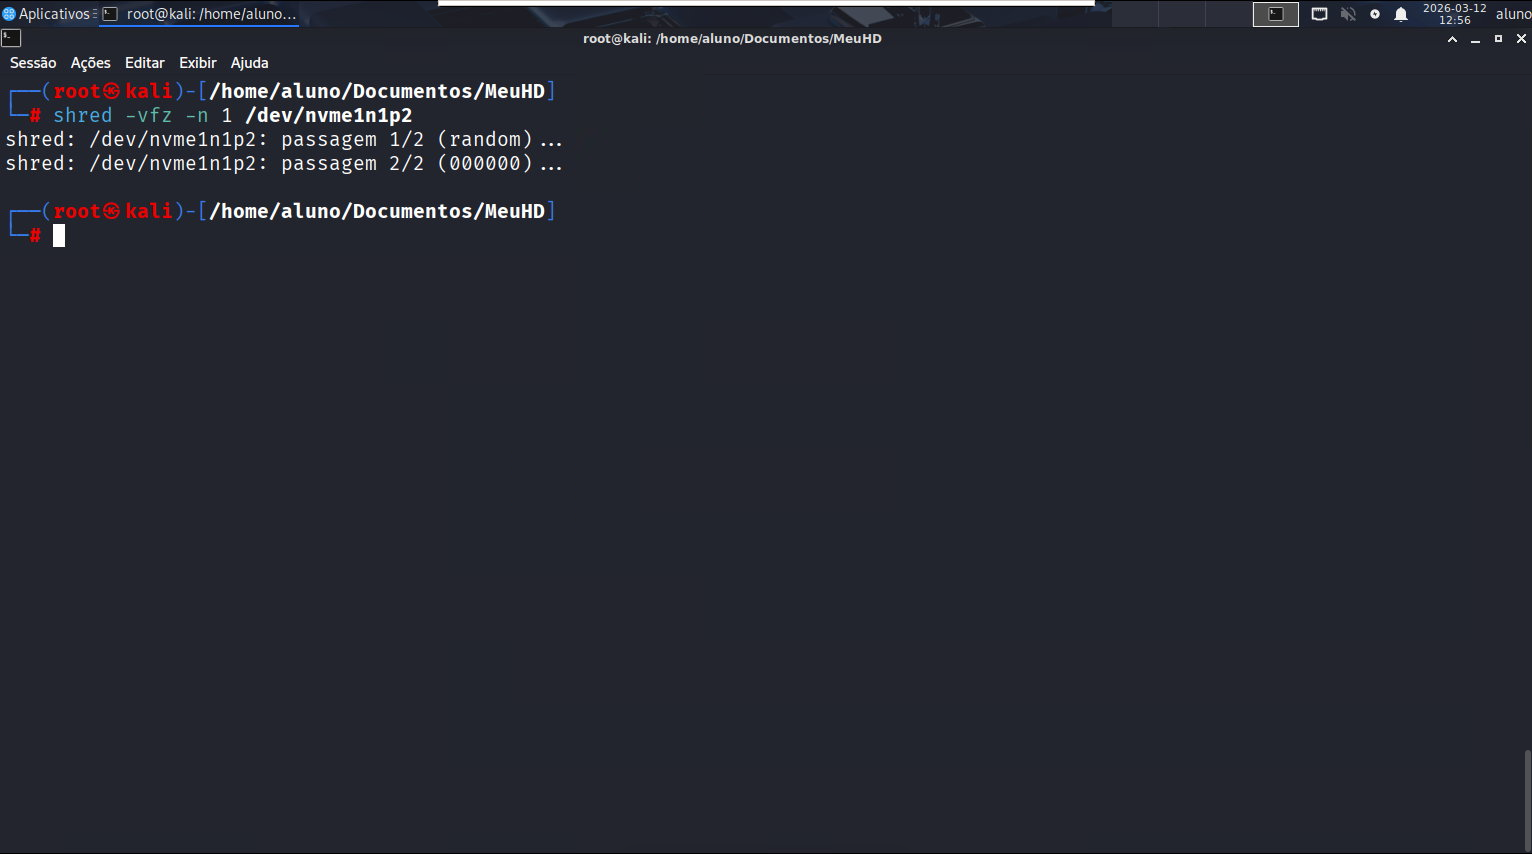
\includegraphics[width=0.99\textwidth]{./fig/fig7.10.png}
  \caption{Execução do comando shred realizando sobrescrita segura da partição}
  \label{fig:fig7.10}
\end{figure}
